%%%%%%%%%%%%%%%%%%%%%%%%%%%%%%%%%%%%%%%%%%%%%%%%%%%%%%%
\section{What to do in the absence of correlations?}

As discussed in Section~\ref{s:correlations}, one doesn't
have to cross-correlate the output of multiple detectors
to search for a stochastic background.
It's just harder if correlation is not an option.
If one knows...

\subsection{LISA}

\begin{figure}[htbp!]
\begin{center}
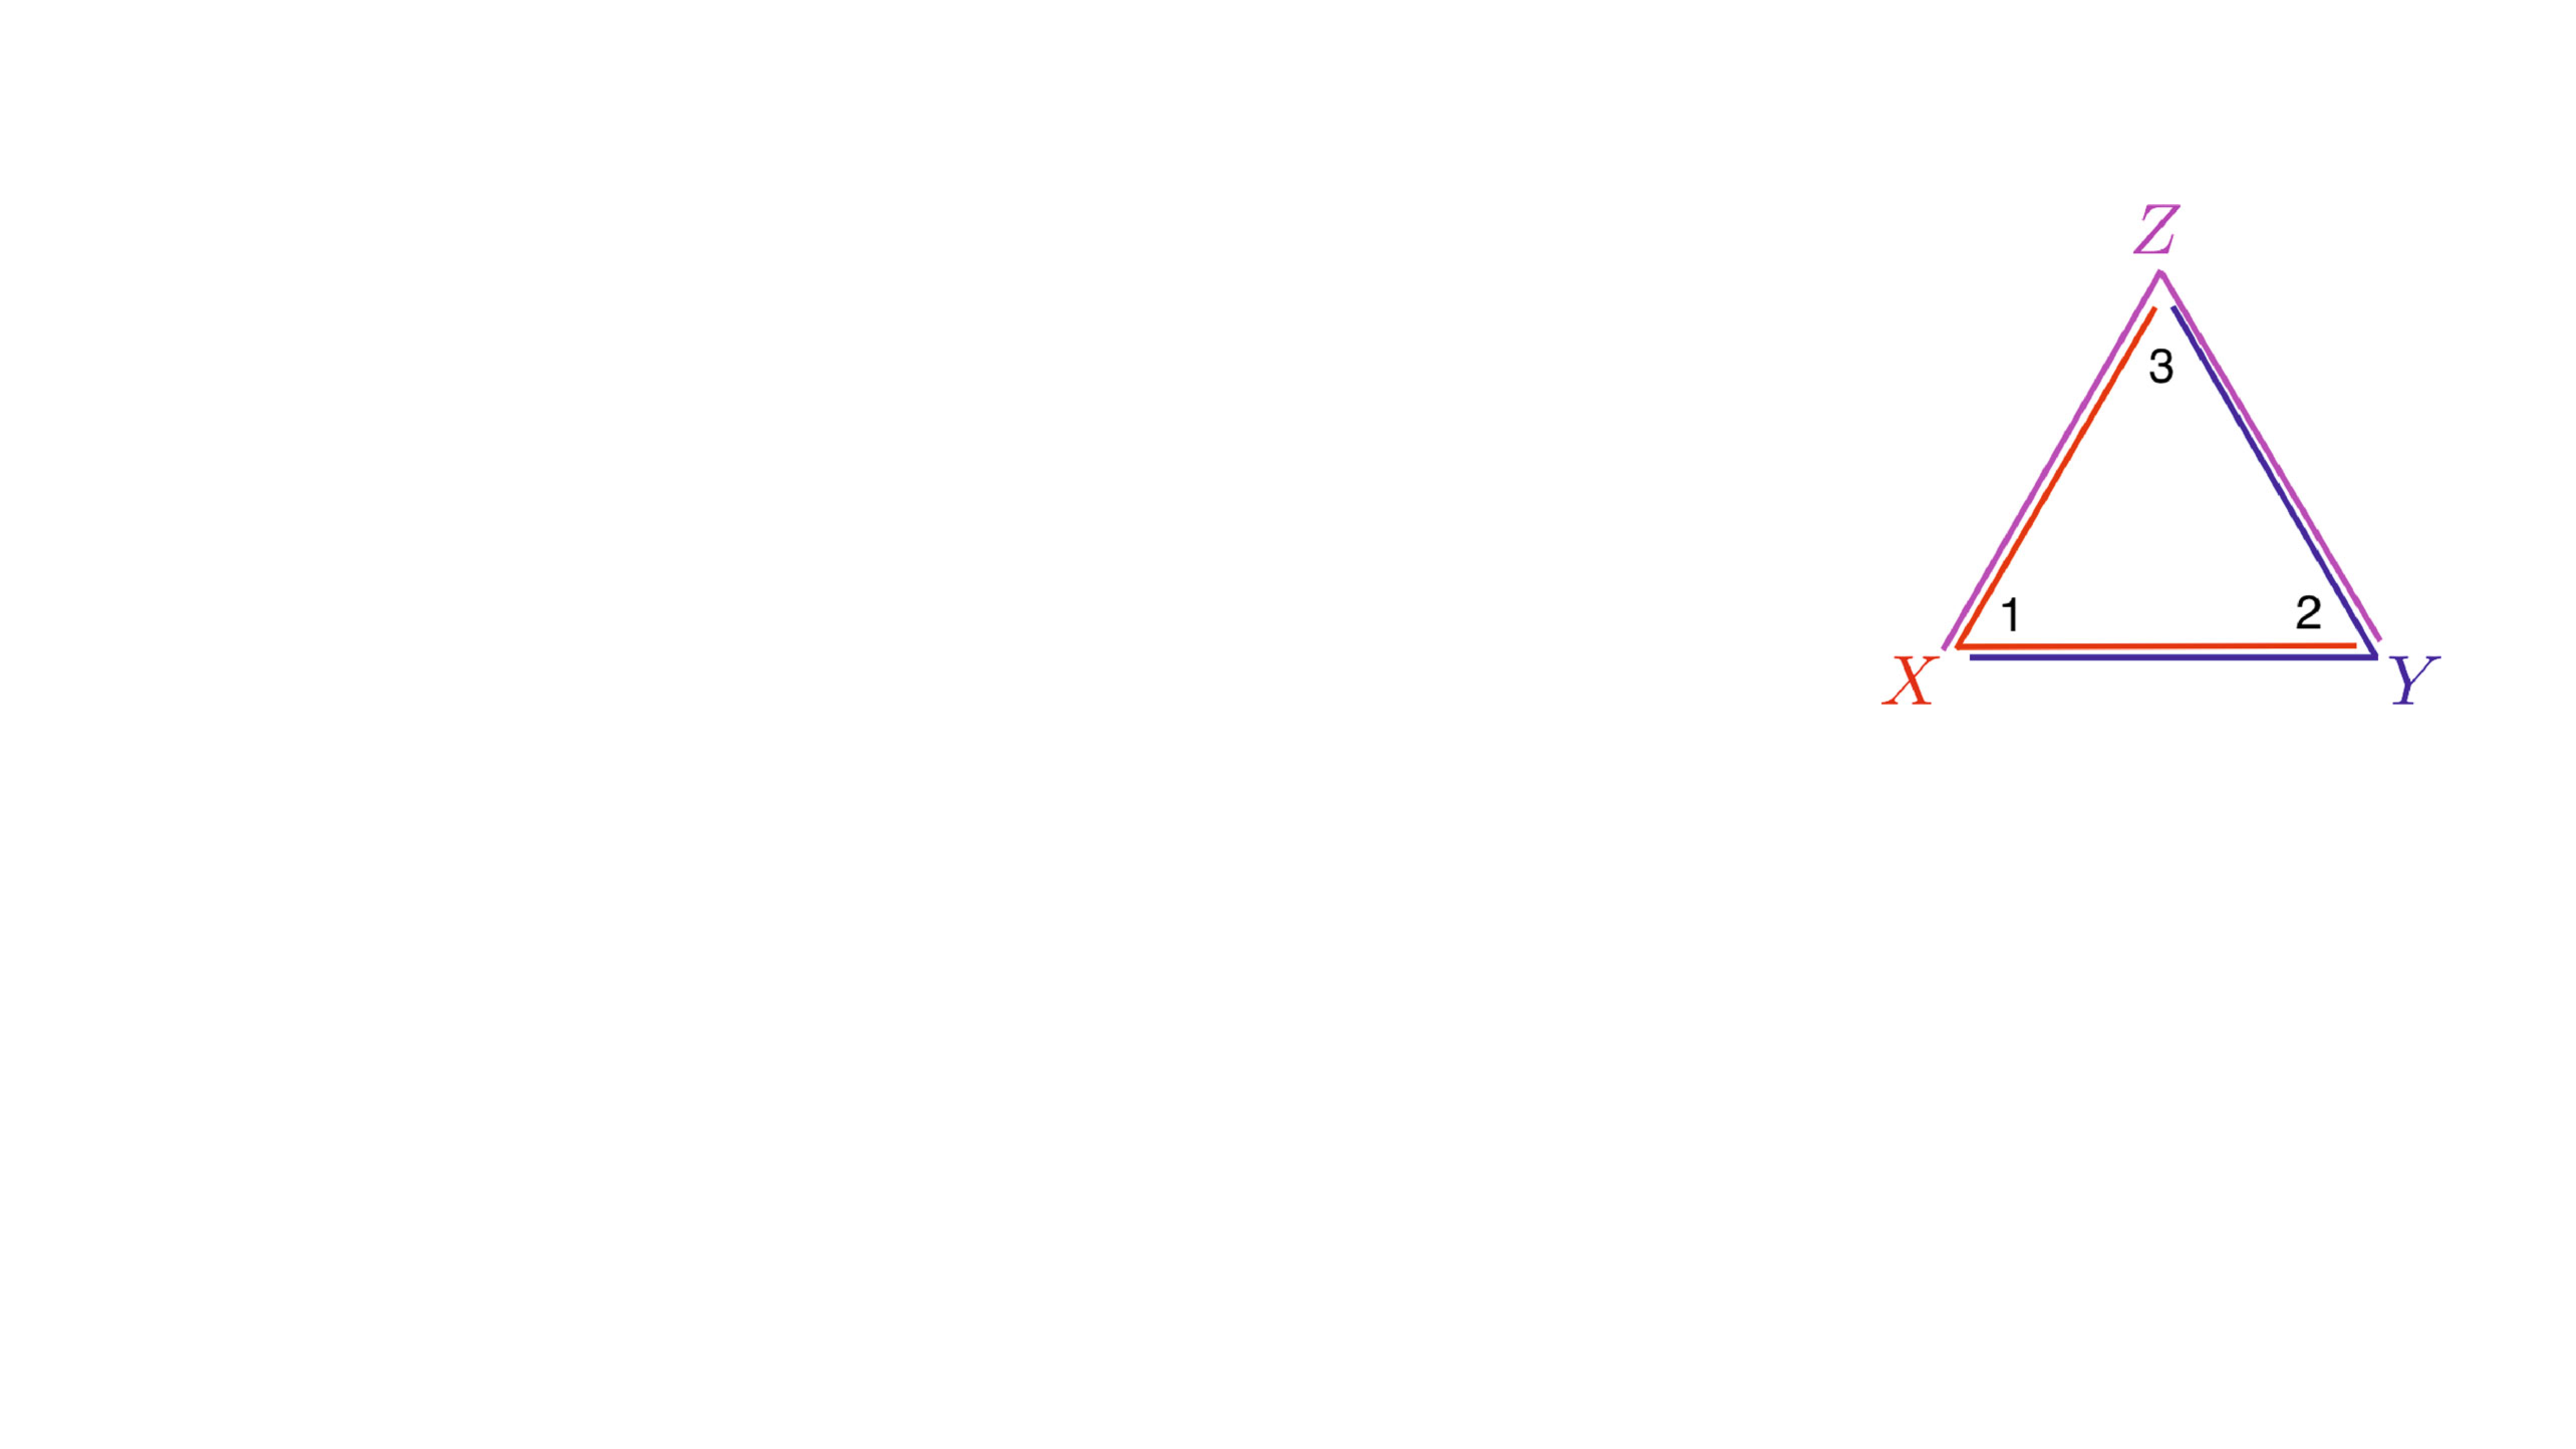
\includegraphics[width=0.3\textwidth]{Figures/LISA_XYZ}
\caption{Schematic representation of the LISA consellation.
$X$, $Y$, $Z$ correspond to Michelson interferometers 
with $60^\circ$ opening angles between the arms, with vertices
located at spacecraft 1, 2, 3.
From $X, Y, Z$, one can construct the TDI combinations
$A, E, T$ described in the text.}
\label{f:LISA_XYZ}
\end{center}
\end{figure}

Although there are 3 Michelson combinations (X,Y,Z), they have common
noise (since they share arms).
Can diagonalize the noise covariance matrix to obtain noise-orthogonal
combinations (A,E,T), which also turn out to be signal orthogonal
%
\be
\begin{aligned}
A&\equiv\frac{1}{3}(2X - Y -Z)\,,
\\
B&\equiv\frac{1}{\sqrt{3}}(Z - Y)\,,
\\
C&\equiv\frac{1}{3}(X+Y+Z)\,,
\end{aligned}
\ee
%
The $A$ and $E$ combinations correspond to the outputs of two 
synthesized Michelson interferometers rotated by $45^\circ$ with
respect to one another.
The Sagnac combination $T$ is relatively insensitive to GW,
at least at lowe frequencies.
Hence it can be used as a {\em null channel}, allowing one to
monitor the instrumental noise.
Nonetheless, proper modeling of instrumental noise, astrophysical
foregrounds (galactic WD binaries), and GWB allows you to discriminate
all three components~\cite{Adams-Cornish:2010, Adams-Cornish:2014}.
\\
\begin{figure}[htbp!]
\begin{center}
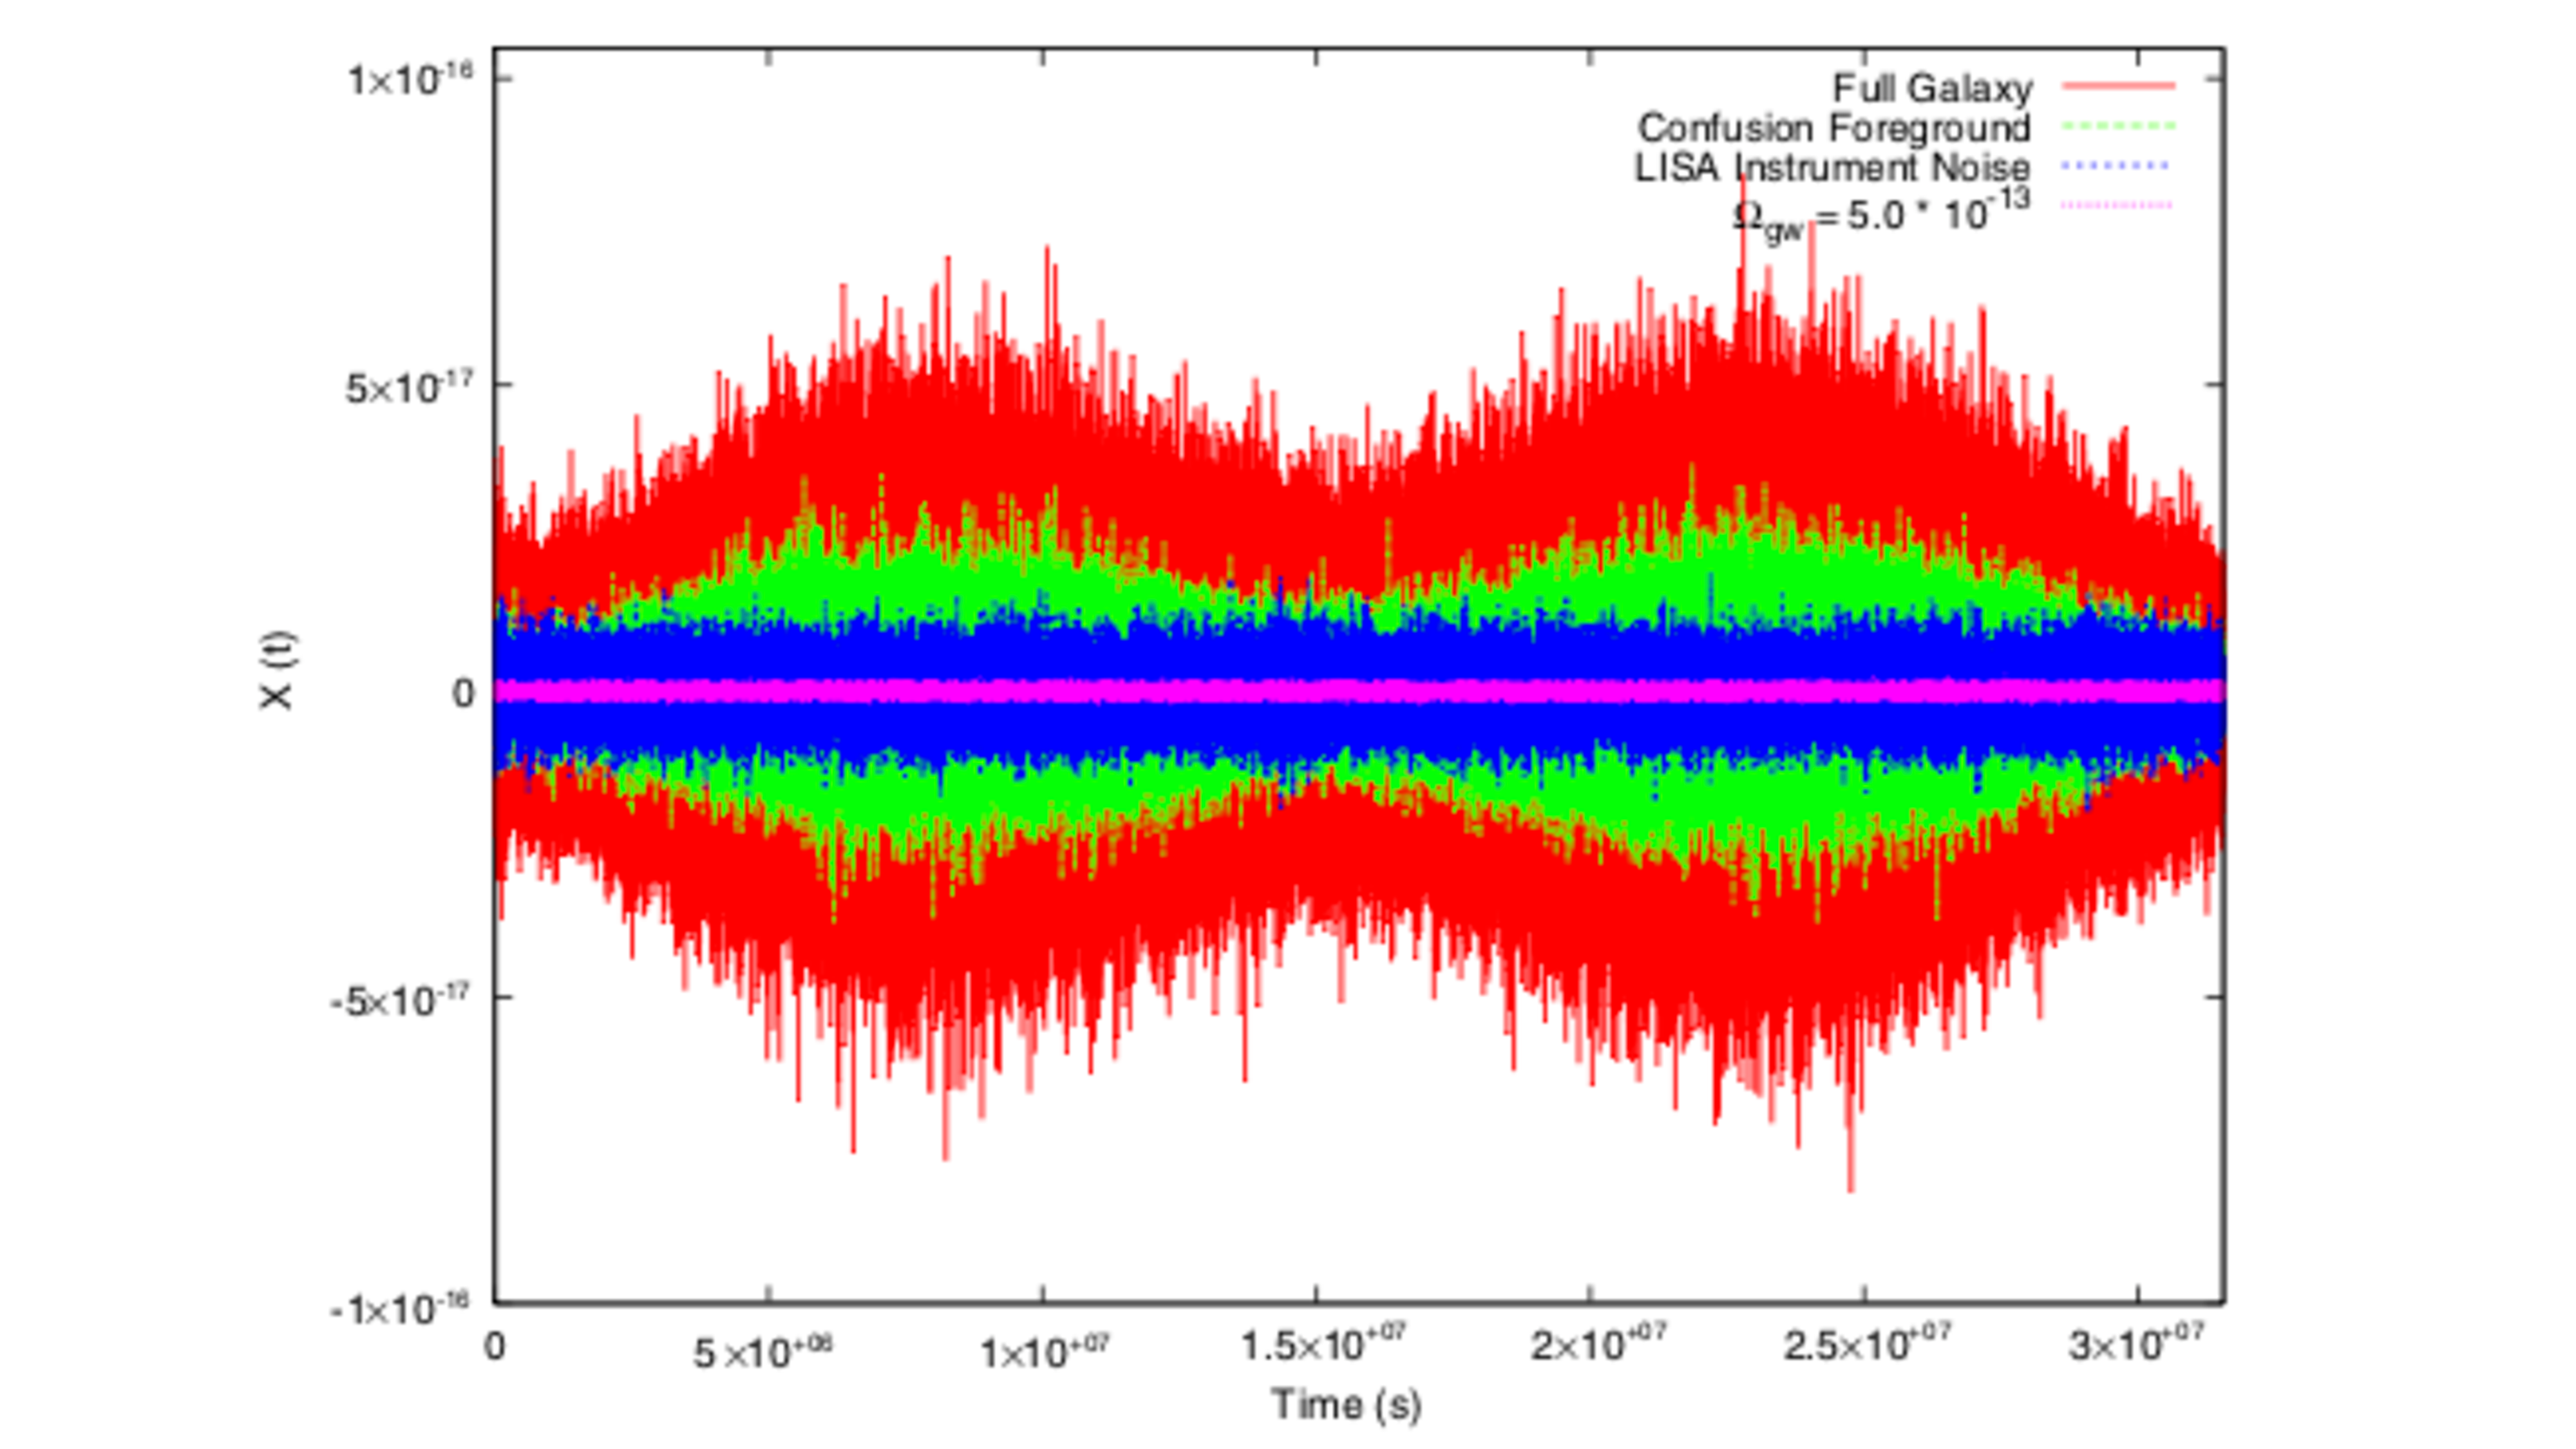
\includegraphics[width=0.7\textwidth]{Figures/LISA_timeseries}
\caption{One-years worth of simulated timeseries data for LISA.
The total output consists of a cosmological GWB (pink);
LISA instrument noise (blue); the full astrophysical foreground
signal from the galactic white-dwarf binary population (red),
which consist of individually resolvable binary signal and 
the confusion-limited foreground (green).
Of particular note are the amplitude and time variability 
of the astrophysical foreground, having a period of 6~months.
Figure taken from \cite{Adams-Cornish:2014}.}
\label{f:LISA_timeseries}
\end{center}
\end{figure}
\begin{figure}[htbp!]

\begin{center}
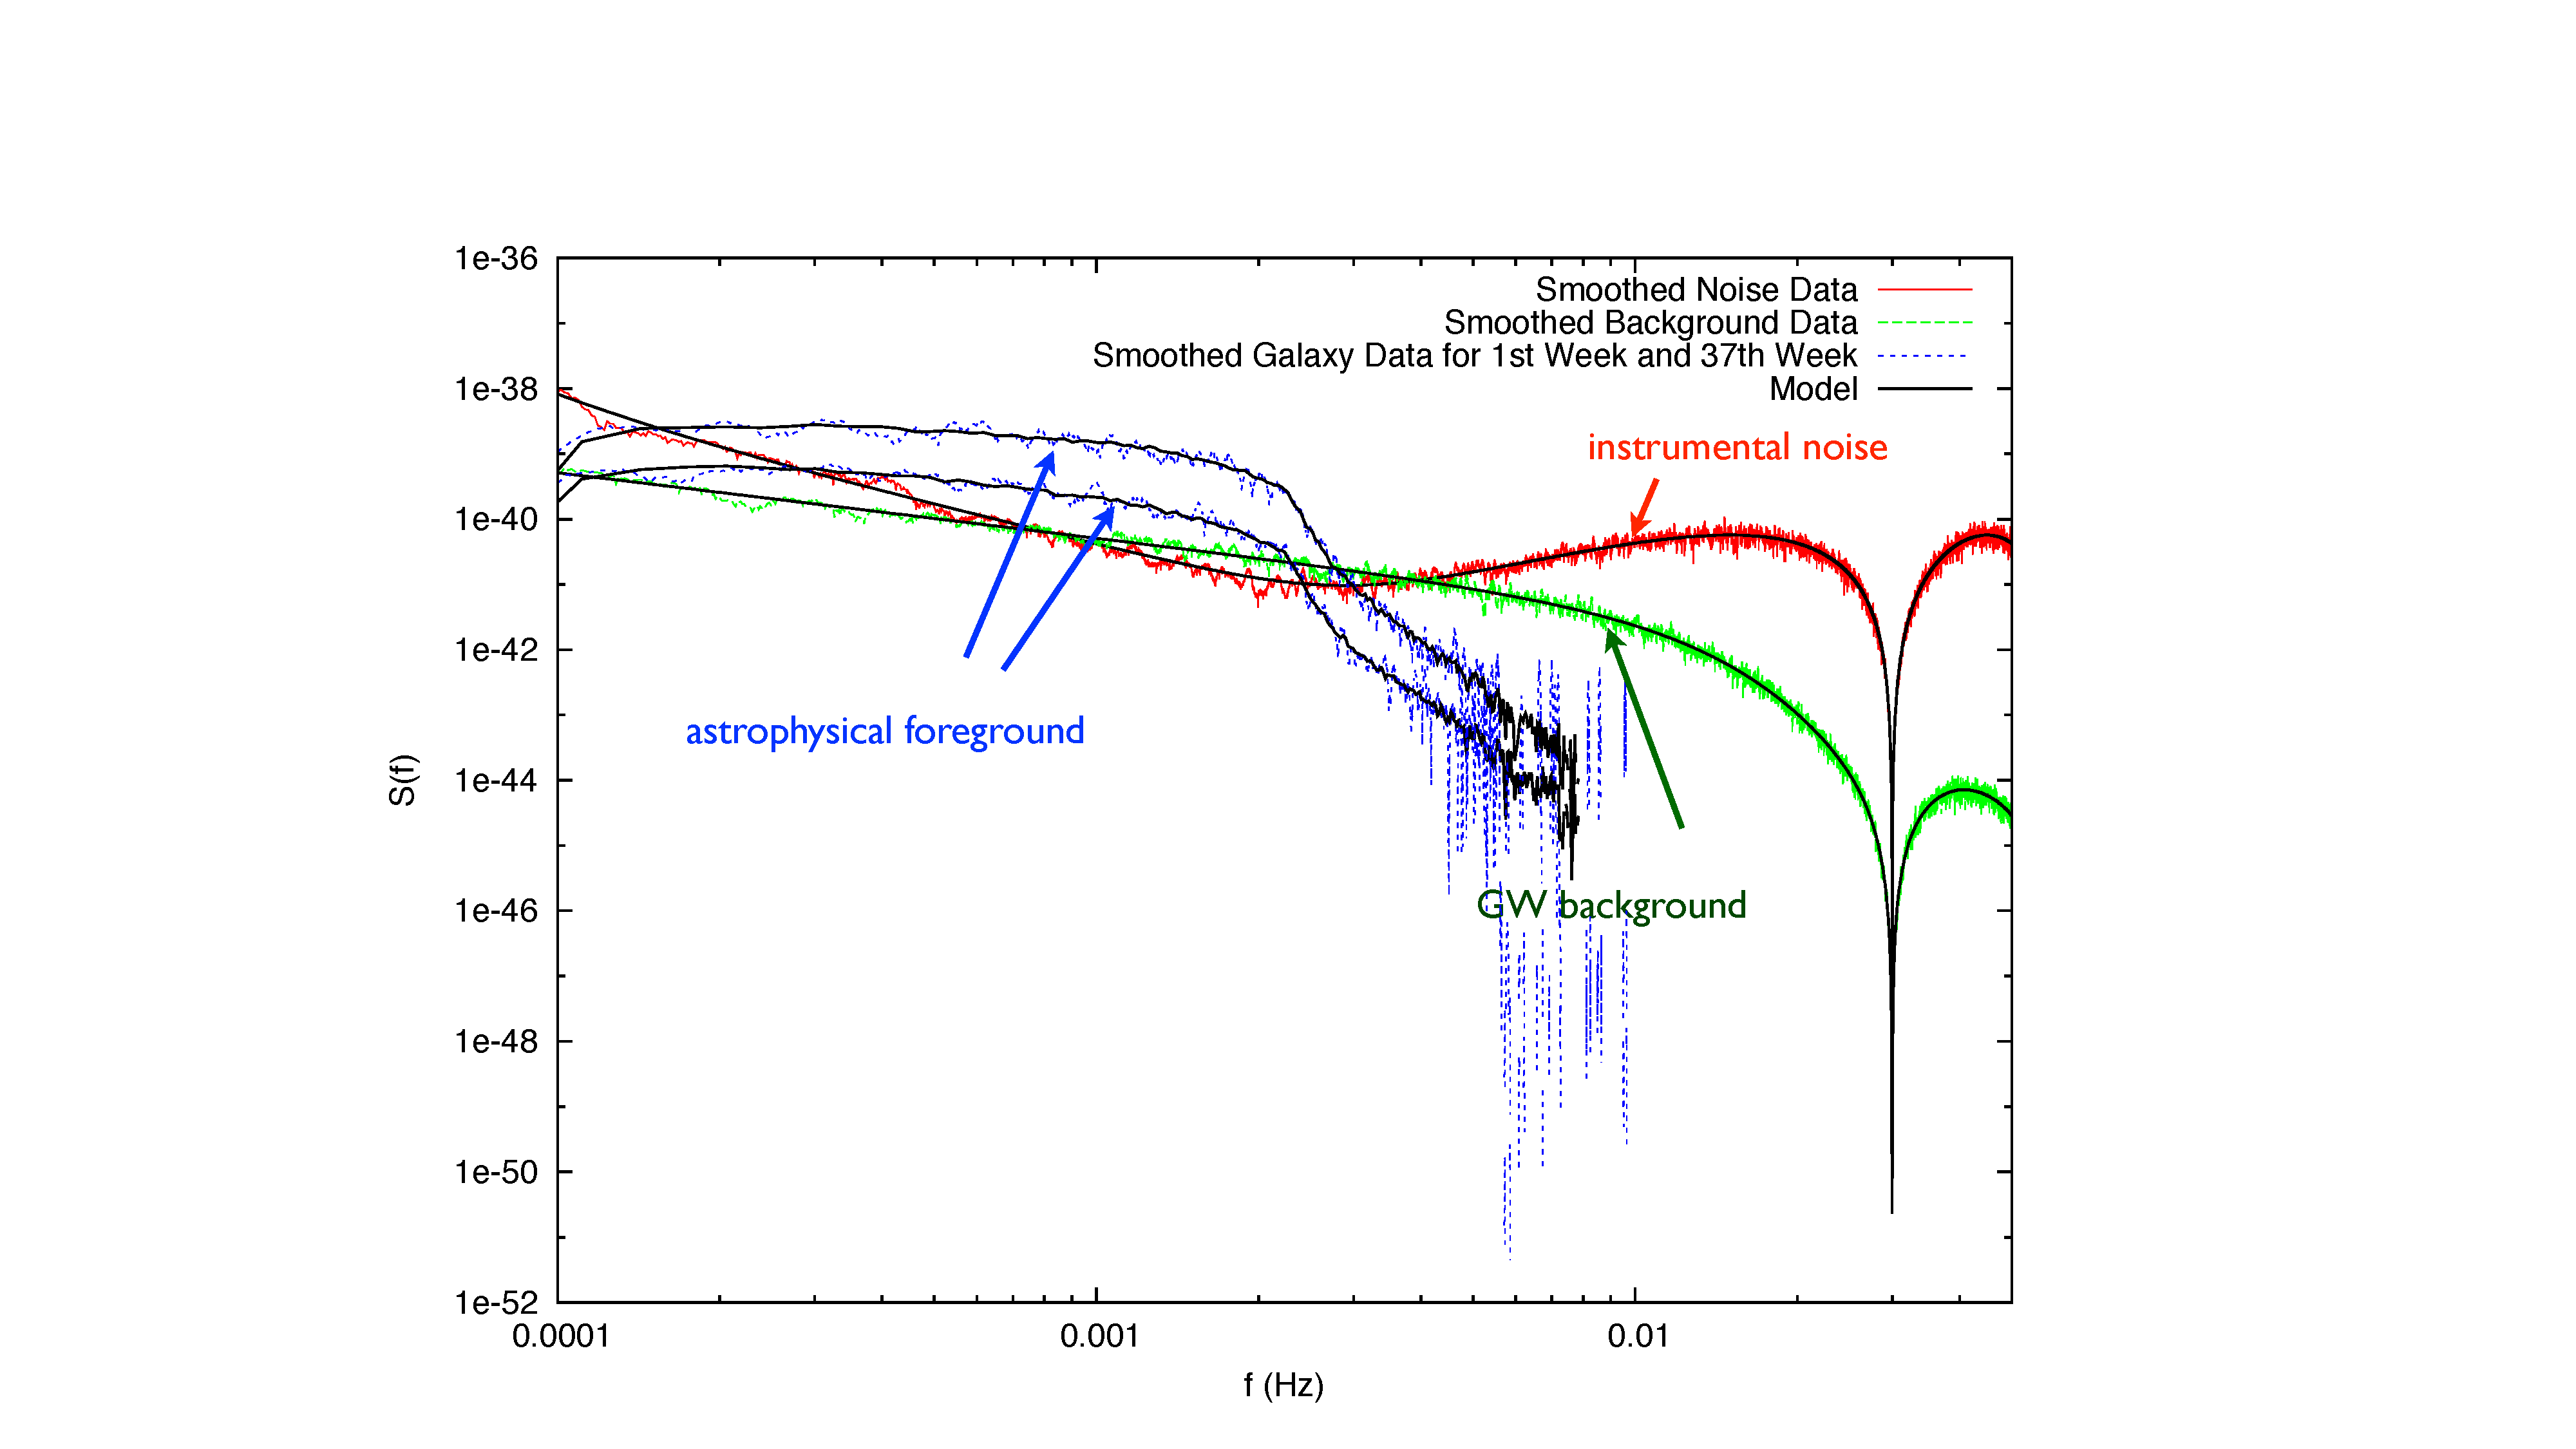
\includegraphics[width=0.6\textwidth]{Figures/LISA_psds}
\caption{Simulated power spectral densities for the 
LISA instrumental noise (red), cosmological GWB (green)
and astrophysical foreground from galactic white dwarf
binaries (blue), the latter at two times during LISAs orbit.
Note the strength of the astrophyical foreground relative
to the instrumental noise, and the different spectral shapes
for the three different contributions.
Figure taken from \cite{Adams-Cornish:2014}.}
\label{f:LISA_psds}
\end{center}
\end{figure}

